\documentclass[pdftex,12pt,a4paper]{report}

\usepackage[pdftex]{graphicx}
\usepackage{float}
\usepackage{fancyvrb}
\fvset{xleftmargin=2em}
\usepackage{graphicx}

\usepackage{pgfplots}
\pgfplotsset{width=10cm,compat=1.9}
\usepackage{tikzscale}
\usepackage{pgfplotstable}
\usepackage{booktabs}
\usepackage[font=small,labelfont=bf,tableposition=top]{caption}

\usepackage[utf8]{inputenc} % isto é um comentário
\usepackage[portuges]{babel}
\usepackage[T1]{fontenc}
\usepackage{times}
%\usepackage{lmodern}
\usepackage[obeyspaces,spaces]{url}
\usepackage[left=25mm,right=25mm,top=25mm,bottom=25mm]{geometry}
\usepackage{titlesec}
\usepackage{mathtools}
%identa 1º paragrafo de capitulos e secções
\usepackage{indentfirst}

\newcommand{\HRule}{\rule{\linewidth}{0.5mm}}
\titleformat{\chapter}{\normalfont\huge}{\thechapter.}{20pt}{\huge}


\begin{document}

\begin{titlepage}


\begin{minipage}{0.3\textwidth}
\begin{flushleft} 

\includegraphics[width=\textwidth]{logo.png}
\end{flushleft}
\end{minipage}
\begin{minipage}{0.6\textwidth}
\begin{flushright} 

\textsc{Departamento de Engenharia Informática}\\[0.1cm]
\bfseries Mestrado Integrado em Engenharia Informática \\ [0.1cm]
\bfseries \textit{Laboratórios de Informática III}\\[8mm]

\end{flushright}
\end{minipage}


\vspace{3cm}


\begin{center}


\LARGE Gestão de Vendas de uma cadeia de Distribuição com 3 filiais

\Large \textbf{GEREVENDAS}\\[1.5cm]


{\Large \bfseries Grupo 84\\[2cm] }


\noindent\begin{minipage}[b]{.1\textwidth}
	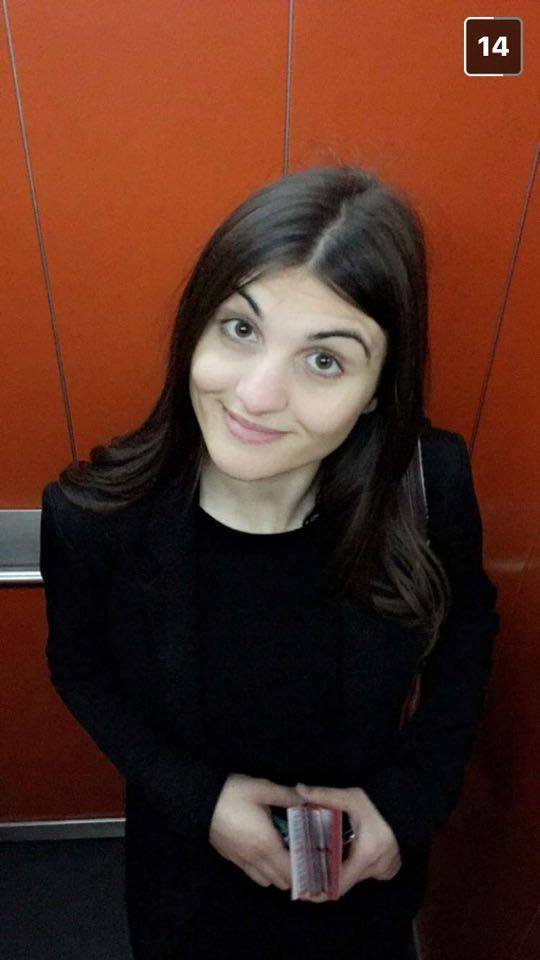
\includegraphics[scale=0.12123]{celia}
	\small{Célia Figueiredo a67637}
\end{minipage} 
\hfill
\begin{minipage}[b]{.1\textwidth}
	
\includegraphics[scale=0.1]{gil}
	\small{Gil Gonçalves a67738}
\end{minipage}
\hfill
\begin{minipage}[b]{.1\textwidth}
	
\includegraphics[scale=0.1]{humberto}
	\small{Humberto Vaz a73236 }
\end{minipage} 
\hfill
\begin{minipage}[b]{.1\textwidth}	
\includegraphics[scale=0.1]{ricardo}
		\small{Ricardo Lopes a72062}
\end{minipage}



\vspace{3ex}


\vfill

\large Braga, {\large \today}

\end{center}
\end{titlepage}


\tableofcontents


\end {document}


